\section{Adding notes}\label{sec:music-notes}
\subsection{Commands for notes}\label{sec:music-notes:commands}
\subsubsection{Note values}\label{sec:music-notes:commands:note-values}
\begin{figure}[t]
  \centering
  \caption{Note value -- the letter part}
  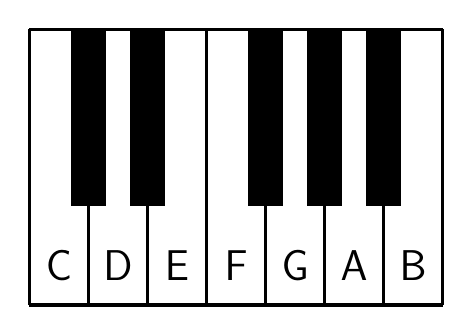
\begin{tikzpicture}[y=1cm/1.5,scale=0.75,transform shape]
    \draw[very thick,fill=white] (0,0) grid[xstep=1,ystep=7] (7,7);
    \foreach \i in {1,2,4,5,6}
      \fill (\i-.3,2.5) rectangle (\i+.3,7);
    \foreach \i [count=\j] in {C,D,E,F,G,A,B}
      \path (\j-.5,1) node[font=\huge\sffamily] {\i};
  \end{tikzpicture}
  \label{fig:music-notes:commands:note-values:letter}
\end{figure}
\begin{figure}[t]
  \centering
  \caption{Note value -- the number part}
  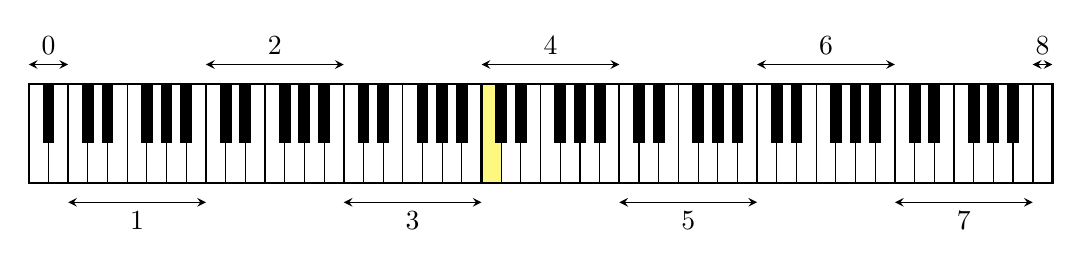
\begin{tikzpicture}[x=0.25cm,y=0.25cm,>=stealth]
    \fill[yellow!50] (23,0) rectangle (24,5);
    \draw (0,0) grid[xstep=1,ystep=5] (52,5);
    \draw[thick,shift={(2,0)}] (0,0) grid[xstep=7,ystep=5] (49,5);
    \draw[thick] (0,0) rectangle (2,5) (51,5) rectangle (52,0);
    \foreach \i in {1,...,7} {
      \foreach \j in {1,2,4,5,6} {
        \fill[shift={({2+(\i-1)*7},0)}] (\j-.3,2) rectangle (\j+.3,5);
      }
    }
    \fill (.7,2) rectangle (1.3,5);
    \foreach \i in {1,...,7} {
      \ifodd\i
        \draw[<->] ({(\i-1)*7+2},-1) -- ++ (7,0) node[midway,below] {\i};
      \else
        \draw[<->] ({(\i-1)*7+2},6) -- ++ (7,0) node[midway,above] {\i};
      \fi
    }
    \draw[<->] (0,6) -- (2,6) node[midway,above] {0};
    \draw[<->] (51,6) -- (52,6) node[midway,above] {8};
  \end{tikzpicture}
  \label{fig:music-notes:commands:note-values:number}
\end{figure}
Every white note is assigned to a `value', which is the \emph{scientific pitch 
notation} of that note. These values have two parts: the letter part and the 
number part:
\begin{itemize}
  \item The letter part can have seven values: |A|, |B|, |C|, \dots, |G|, 
  indicating the name of the note (\emph{do}, \emph{re}, \emph{mi}, \dots). (See 
  figure \ref{fig:music-notes:commands:note-values:letter}).
  \item The number part is a whole number between $0$ to $8$, indicating which 
  octave the note is in. (See figure \ref{fig:music-notes:commands:note-values:number}).
\end{itemize}
For example, \emph{F\"ur Elise} by Beethoven starts with an |E5| (a \emph{mi} at the 
5th octave).

We will only work with these values. To have black notes in your score, you can 
use |\tmappendaccidental| to add the accidentals.

The package will automatically detect which staff you are using, when you use 
these values.
\subsubsection{Note names}\label{sec:music-notes:commands:note-names}
It is very possible that a note will be refered to later in the staff (to add 
notations to it, etc.). In this package, to refer to notes, we will use note 
\emph{names}. Just like \tikzname\ node names, etc. -- you can leave the name 
empty if you want, but you will not be able to communicate with that unnamed note 
any time later in the document.
\subsubsection{Whole notes}\label{sec:music-notes:commands:whole}
\begin{command}{\tmwhole\opt{\oarg{options}}\marg{x-pos}\marg{note value list}\marg{name}}
  Add a set of whole notes at $x$-position \meta{x-pos}. Each value in the 
  comma-separated list \meta{note value list} corresponds to a note.

  \meta{name} can be left empty, but as in the staff naming, I strongly advise 
  you to find some name for each note set.

  The center of note with note value $x$ will be marked as coordinate 
  |(|\meta{name}|-|$x$|)|. For example, note |F5| will be marked as 
  |(|\meta{name}|-F5)|. Also, the point on the middle line of the staff which is 
  at \meta{x-pos} will be marked as |(|\meta{name}|-center)|.
\end{command}
\begin{codeexample}[]
\begin{tmline}
\begin{tmstaff}{g}{}
  \tmwhole{3}{C4,E4,G4}{c-major}\tmwhole{5}{A4,C5,E5}{a-minor}
\end{tmstaff}
\end{tmline}
\end{codeexample}
\subsubsection{Relative positioning}\label{sec:music-notes:commands:relative}
Consider the following example:
\begin{codeexample}[]
\begin{tmline}
\begin{tmstaff}{g}{}
  \tmwhole{5}{D4,F4,G4}{}% G7
\end{tmstaff}
\end{tmline}
\end{codeexample}
It looks very bad, doesn't it? Note |G4| should be shifted a bit to the right. 
You can achieve this by using the following key:
\begin{key}{/tm/relative=\meta{relative position} (initially center)}
  Apply relative position to the note. \meta{relative position} can be either 
  |center|, |left| or |right|.
\end{key}
The option applies to every note inside a command like |\tmwhole|, so you 
occasionally need to have two or three different |\tmwhole|s at the same position:
\begin{codeexample}[]
\begin{tmline}
\begin{tmstaff}{g}{}
  \tmwhole{5}{D4,G4}{}\tmwhole[relative=right]{5}{F4}{}
\end{tmstaff}
\end{tmline}
\end{codeexample}
Note that if the note is not a whole note, i.e. it has a stem, and it is not 
beamed, i.e. it is created with |\tmhalf|, |\tmquarter|, etc., the stem will only 
be drawn if |relative=center|.
\subsubsection{Half notes}\label{sec:music-notes:commands:half}
\begin{command}{\tmhalf\opt{\oarg{options}}\marg{x-pos}\marg{note value list}\marg{name}}
  Add a half note at position \meta{x-pos}. The stem direction will be automatically 
  determined.
\end{command}
The end of the stem is marked as coordinate |(|\meta{name}|-tail)|. (This also 
applies to |\tmquarter|, |\tmeighth| and |\tmmorethaneighth|.)
\begin{codeexample}[]
\begin{tmline}%
\begin{tmstaff}{g}{}
  \tmhalf{2}{E4}{}\tmhalf{3}{F5}{}\tmhalf{4}{E4,F5}{}\tmhalf{5}{B4}{}
  \tmhalf[reversed]{6}{E4}{}      \tmhalf[reversed]{7}{F5}{}
  \tmhalf[reversed]{8}{E4,F5}{}   \tmhalf[reversed]{9}{B4}{}
  \tmhalf{11}{B4,G4}{}            \tmhalf[relative=right]{11}{C5}{}
  \tmhalf[reversed]{11}{G4}{}     \tmhalf[reversed,relative=left]{11}{F4}{}
\end{tmstaff}%
\end{tmline}
\end{codeexample}
\subsubsection{Stem direction}\label{sec:music-notes:commands:stem-direction}
You can change the default direction of the stem by using the following key:
\begin{key}{/tm/reversed=\meta{|true| or |false|} (default true)}
  If this is set to |true|, the stem direction of |\tmhalf|, |\tmquarter|, \dots 
  will be reversed. If this key is applied to |\tmslur|, the direction of the 
  slur will be reversed (see more in section \ref{sec:line:slur}).
\end{key}
\begin{codeexample}[]
\begin{tmline}
\begin{tmstaff}{g}{}
  \tmhalf{3}{C5}{}\tmhalf[reversed]{6}{C5}{}
\end{tmstaff}
\end{tmline}
\end{codeexample}
\subsubsection{Quarter notes}\label{sec:music-notes:commands:quarter}
\begin{command}{\tmquarter\opt{\oarg{options}}\marg{x-pos}\marg{note value list}\marg{name}}
  Similar to |\tmhalf|.
\end{command}
\begin{codeexample}[]
\begin{tmline}%
\begin{tmstaff}{g}{}
  \tmquarter{2}{E4}{}\tmquarter{3}{F5}{}\tmquarter{4}{E4,F5}{}\tmquarter{5}{B4}{}
  \tmquarter[reversed]{6}{E4}{}         \tmquarter[reversed]{7}{F5}{}
  \tmquarter[reversed]{8}{E4,F5}{}      \tmquarter[reversed]{9}{B4}{}
  \tmquarter{11}{B4,G4}{}               \tmquarter[relative=right]{11}{C5}{}
  \tmquarter[reversed]{11}{G4}{}        \tmquarter[reversed,relative=left]{11}{F4}{}
\end{tmstaff}%
\end{tmline}
\end{codeexample}
\subsubsection{Eighth notes}\label{sec:music-notes:commands:eighth}
\begin{command}{\tmeighth\opt{\oarg{options}}\marg{x-pos}\marg{note value list}\marg{name}}
  Similar to |\tmhalf|.
\end{command}
\begin{codeexample}[]
\begin{tmline}%
\begin{tmstaff}{g}{}
  \tmeighth {2}{E4}{}\tmeighth{3}{F5}{}\tmeighth{4}{E4,F5}{}\tmeighth{5}{B4}{}
  \tmeighth[reversed]{6}{E4}{}         \tmeighth[reversed]{7}{F5}{}
  \tmeighth[reversed]{8}{E4,F5}{}      \tmeighth[reversed]{9}{B4}{}
  \tmeighth{11}{B4,G4}{}               \tmeighth[relative=right]{11}{C5}{}
  \tmeighth[reversed]{11}{G4}{}        \tmeighth[reversed,relative=left]{11}{F4}{}
\end{tmstaff}%
\end{tmline}
\end{codeexample}
\subsubsection{More than eighth notes}\label{sec:music-notes:commands:more-than-eighth}
The commands described in this section applies to every notes below the eighth 
notes, including the sixteenth note (semiquaver), the thirty-second note 
(demisemiquaver), etc.
\begin{command}{\tmmorethaneighth\opt{\oarg{options}}\marg{x-pos}\marg{note value list}\marg{number of flags}\marg{name}}
  Similar to |\tmhalf|.
\end{command}
\begin{codeexample}[]
\begin{tmline}%
\begin{tmstaff}{g}{}
  \tmmorethaneighth{2}{F4}{2}{note-2}
  \tmmorethaneighth{3}{F4}{3}{note-3}
  \tmmorethaneighth{4}{F4}{4}{note-4}
  \tmmorethaneighth{5}{F4}{5}{note-5}
  \tmmorethaneighth{6}{F4}{6}{note-6}
\end{tmstaff}%
\end{tmline}
\end{codeexample}
\subsection{Beaming}\label{sec:music-notes:beam}
\begin{environment}{{tmbeam}\opt{\oarg{options}}}
  Add a beaming note series. All notes inside this environment are `beamed' 
  together, and all stems point {\bfseries upwards}.
\end{environment}
\begin{environment}{{tmbeam*}\opt{\oarg{options}}}
  Identical to |{tmbeam}|, only all stems point {\bfseries downwards}.
\end{environment}
\emph{All} notes to be beamed inside these environments need to be added using 
the following command (|\tmeighth|, \dots\ will simply not work):
\begin{command}{\tmbeamnote\opt{\oarg{options}}\marg{x-pos}\marg{note value}\marg{number of flags}\marg{name}}
  Add a note to the beaming series. If \meta{number of flags} is $1$, it is an 
  eighth note, if \meta{number of flags} is $2$, it is a sixteenth note, and so 
  on.
\end{command}
{\bfseries\sffamily Important note:} Because of the algorithm working 
behind the scene, you \emph{must} give a separate name to each |\tmbeamnote| 
inside |{tmbeam}| or |{tmbeam*}|. Doing otherwise will result in 
weird output.
\begin{codeexample}[]
\begin{tmline}%
\begin{tmstaff}{g}{p1}
  \tmtimesignature{1}{3}{8}
  \begin{tmbeam*}
    \tmbeamnote{1.75}{E5}{2}{}\tmbeamnote{2.5}{D5}{2}{a}
    \tmappendaccidental{a}{D5}{sharp}
  \end{tmbeam*}
  \tmbarlineinline{2.8}
  \begin{tmbeam*}
    \tmbeamnote{3.25}{E5}{2}{a}\tmbeamnote{4}{D5}{2}{b}\tmbeamnote{4.5}{E5}{2}{c}
    \tmbeamnote{5}{B4}{2}{d}\tmbeamnote{5.5}{D5}{2}{e}\tmbeamnote{6}{C5}{2}{f}
    \tmappendaccidental{b}{D5}{sharp}\tmappendaccidental{e}{D5}{natural}
  \end{tmbeam*}
  \tmbarlineinline{6.3}\tmeighth{6.75}{A4}{a}\tmadddot{a}{1}
  \begin{tmbeam}
    \tmbeamnote{8}{C4}{2}{a}\tmbeamnote{8.5}{E4}{2}{b}\tmbeamnote{9}{A4}{2}{c}
  \end{tmbeam}
  \tmbarlineinline{9.3}\tmeighth{9.75}{B4}{a}\tmadddot{a}{1}
  \begin{tmbeam}
    \tmbeamnote{10.75}{E4}{2}{a}\tmbeamnote{11.5}{G4}{2}{b}\tmbeamnote{12}{B4}{2}{c}
    \tmappendaccidental{b}{G4}{sharp}
  \end{tmbeam}
  \tmbarlineinline{12.3}\tmquarter{12.75}{C5}{a}\tmadddot{a}{1}
\end{tmstaff}%
\tmbarlineendline{p1}{p1}%
\end{tmline}
\end{codeexample}
\subsection{Commands for rests}\label{sec:music-notes:rests}
This package currently provides support for the following rests:
\begin{command}{\tmwholerest\opt{\oarg{options}}\marg{x-pos}}
  Add a whole rest at $x$-position \meta{x-pos}.
\end{command}
\begin{command}{\tmhalfrest\opt{\oarg{options}}\marg{x-pos}}
  Add a half rest at $x$-position \meta{x-pos}.
\end{command}
\begin{command}{\tmquarterrest\opt{\oarg{options}}\marg{x-pos}}
  Add a quarter rest at $x$-position \meta{x-pos}.
\end{command}
\begin{command}{\tmbelowquarterrest\opt{\oarg{options}}\marg{x-pos}\marg{number}}
  Add a rest at $x$-position \meta{x-pos}, whose value is below a quarter rest. 
  The rest has \meta{number} `flags': if \meta{number} is $1$, it is an eighth 
  rest, if \meta{number} is $2$, it is a sixteenth rest, and so on... Currently 
  \meta{number} must be an integer between |1| and |4|.
\end{command}
\begin{command}{\tmeighthrest\opt{\oarg{options}}\marg{x-pos}}
  Identical to |\tmbelowquarterrest| where \meta{number} is $1$.
\end{command}
\begin{command}{\tmsixteenthrest\opt{\oarg{options}}\marg{x-pos}}
  Identical to |\tmbelowquarterrest| where \meta{number} is $2$.
\end{command}
\begin{command}{\tmthirtysecondrest\opt{\oarg{options}}\marg{x-pos}}
  Identical to |\tmbelowquarterrest| where \meta{number} is $3$.
\end{command}
\begin{command}{\tmsixtyfourthrest\opt{\oarg{options}}\marg{x-pos}}
  Identical to |\tmbelowquarterrest| where \meta{number} is $4$.
\end{command}
\begin{codeexample}[]
\begin{tmline}%
\begin{tmstaff}{g}{}
  \tmwholerest{2}\tmhalfrest{4}\tmquarterrest{6}
\end{tmstaff}%
\begin{tmstaff}{g}{}
  \tmbelowquarterrest{2}{1}\tmeighthrest{3}
  \tmbelowquarterrest{4}{2}\tmsixteenthrest{5}
  \tmbelowquarterrest{6}{3}\tmthirtysecondrest{7}
  \tmbelowquarterrest{8}{4}\tmsixtyfourthrest{9}
\end{tmstaff}%
\end{tmline}
\end{codeexample}
\subsection{Miscellaneous}\label{sec:music-notes:misc}
\subsubsection{Accidentals}\label{sec:music-notes:misc:accidentals}
\begin{command}{\tmappendaccidental\opt{\oarg{options}}\marg{note name}\marg{note value}\marg{type}}
  Add accidental \meta{type} to note of value \meta{note value} in 
  \meta{note name}. \meta{type} can have five values: |sharp|, |flat|, 
  |double-sharp|, |double-flat| and |natural|.
\end{command}
\begin{codeexample}[]
\begin{tmline}%
\begin{tmstaff}{g}{}
  \tmquarter{2}{B4}{a}\tmquarter{3}{B4}{b}\tmquarter{4}{B4}{c}
  \tmquarter{5}{B4}{d}\tmquarter{6}{B4}{e}\tmquarter{9}{E4,G4,B4}{f}
  \tmappendaccidental{a}{B4}{sharp}
  \tmappendaccidental{b}{B4}{double-sharp}
  \tmappendaccidental{c}{B4}{flat}
  \tmappendaccidental{d}{B4}{double-flat}
  \tmappendaccidental{e}{B4}{natural}
  \tmappendaccidental{f}{E4}{sharp}
  \tmappendaccidental[xshift=-2mm]{f}{G4}{sharp}
  \tmappendaccidental[xshift=-4mm]{f}{B4}{sharp}
\end{tmstaff}%
\end{tmline}
\end{codeexample}
\subsubsection{Dots}\label{sec:music-notes:misc:dots}
\begin{command}{\tmadddot\opt{\oarg{options}}\marg{note name}\marg{number of dots}}
  Add \meta{number of dots} dot to note in \meta{note name}. 
\end{command}
\begin{codeexample}[]
\begin{tmline}%
\begin{tmstaff}{g}{}
  \tmquarter{4}{F4,A4}{a}\tmquarter{6}{G4,B4}{b}\tmquarter{8}{A4,C5}{c}
  \tmadddot{a}{1}\tmadddot{b}{1}\tmadddot{c}{10}
\end{tmstaff}%
\end{tmline}
\end{codeexample}
\subsubsection{Articulations}\label{sec:music-notes:misc:articulations}
\begin{command}{\tmstaccato\opt{\oarg{options}}\marg{note name}}
  Add \emph{staccato} to note \meta{note name}.
\end{command}
\begin{command}{\tmtenuto\opt{\oarg{options}}\marg{note name}}
  Add \emph{tenuto} to note \meta{note name}.
\end{command}
\begin{command}{\tmaccentabove\opt{\oarg{options}}\marg{note name}}
  Add an accent to note \meta{note name} (one form of \emph{marcato}).
\end{command}
\begin{command}{\tmstaccatissimo\opt{\oarg{options}}\marg{note name}}
  Add \emph{staccatissimo} to note \meta{note name}.
\end{command}
\begin{command}{\tmmarcato\opt{\oarg{options}}\marg{note name}}
  Add \emph{marcato} to note \meta{note name}.
\end{command}
\begin{codeexample}[]
\begin{tmline}
\begin{tmstaff}{g}{}
  \tmquarter{2}{B4}{x}\tmstaccato{x}
  \tmquarter{3}{B4}{x}\tmstaccato[line shift=2]{x}
  \tmquarter{4}{B4}{x}\tmtenuto{x}
  \tmquarter{5}{B4}{x}\tmtenuto[line shift=2]{x}
  \tmquarter{6}{B4}{x}\tmaccentabove{x}
  \tmquarter{7}{B4}{x}\tmaccentabove[line shift=1]{x}
  \tmquarter{8}{B4}{x}\tmstaccatissimo{x}
  \tmquarter{9}{B4}{x}\tmstaccatissimo[line shift=1]{x}
  \tmquarter{10}{B4}{x}\tmmarcato{x}
  \tmquarter{11}{B4}{x}\tmmarcato[line shift=1]{x}
\end{tmstaff}
\end{tmline}
\end{codeexample}
For fermatas we have the following two commands:
\begin{command}{\tmfermataabove\opt{\oarg{options}}\marg{note name}}
  Add an `above-fermata' to \meta{note name}.
\end{command}
\begin{command}{\tmfermata\opt{\oarg{options}}\marg{note name}}
  Alias of |\tmfermataabove|.
\end{command}
\begin{command}{\tmfermatabelow\opt{\oarg{options}}\marg{note name}}
  Add a `below-fermata' to \meta{note name}.
\end{command}
\begin{codeexample}[]
\begin{tmline}
\begin{tmstaff}{g}{}
  \tmquarter{5}{C4}{x}\tmfermataabove{x}
  \tmquarter{8}{C4}{x}\tmfermatabelow{x}
\end{tmstaff}
\end{tmline}
\end{codeexample}
\subsubsection{Ornaments}\label{sec:music-notes:misc:ornaments}
\begin{command}{\tmtrill\opt{\oarg{options}}\marg{note name}}
  Add a trill to note \meta{note name}.
\end{command}
\begin{command}{\tmturn\opt{\oarg{options}}\marg{note name}}
  Add a turn to note \meta{note name}.
\end{command}
\begin{command}{\tmuppermordent\opt{\oarg{options}}\marg{note name}}
  Add a `upper' mordent to note \meta{note name}.
\end{command}
\begin{command}{\tmlowermordent\opt{\oarg{options}}\marg{note name}}
  Add an `lower' mordent to note \meta{note name}.
\end{command}
\begin{command}{\tmmordent\opt{\oarg{options}}\marg{note name}}
  Alias of |\tmuppermordent|.
\end{command}
\begin{codeexample}[]
\begin{tmline}
\begin{tmstaff}{g}{}
  \tmquarter{2}{C5}{a}\tmquarter{4}{C5}{b}\tmquarter{6}{C5}{c}\tmquarter{8}{C5}{d}
  \tmtrill{a}\tmturn{b}\tmuppermordent{c}\tmlowermordent{d}
\end{tmstaff}
\end{tmline}
\end{codeexample}
\subsubsection{Tremolo}\label{sec:music-notes:misc:tremolo}
\begin{command}{\tmtremolo\opt{\oarg{options}}\marg{note}\marg{number}}
  Add a tremolo to note \meta{note}.
\end{command}
\begin{command}{\tmtremolocoordinate\opt{\oarg{options}}\marg{coordinate}\marg{number}}
  Add a tremolo to coordinate \meta{coordinate}.
\end{command}
\begin{codeexample}[]
\begin{tmline}
\begin{tmstaff}{g}{}
  \tmquarter{4}{C4}{a}\tmtremolo{a}{1}\tmquarter{7}{D4}{b}\tmtremolo[red]{b}{2}
  \tmtremolocoordinate{5.5,-.55}{2}
\end{tmstaff}
\end{tmline}
\end{codeexample}
